\documentclass[12pt,a4paper]{article}

\usepackage[utf8]{inputenc}
\usepackage[english]{babel}
\usepackage{amsmath}
\usepackage{amsfonts}
\usepackage{amssymb}
\usepackage{graphicx}
\usepackage{mathtools}
\usepackage{amsfonts}
\usepackage{pdfpages}
\usepackage{hyperref}
\usepackage{cite}
\usepackage{subfig}
\usepackage[left=2cm,right=2cm,top=2cm,bottom=2cm]{geometry}
\everymath{\displaystyle}
\author{Boyan Naydenov}
\title{Boundary Value Problem \textit{BVP}. Assignment 1a}


\begin{document}
\begin{titlepage}
	\centering
	\vspace{4.5cm}
	{\scshape ESEIAAT \par}
	{\scshape\Large \par}
	\vspace{1.5cm}
	{\huge\bfseries ASTREA Ground Station design \par}
	\vspace{10cm}
	\vspace{3cm}
	{\Large\itshape Boyan Naydenov\par}
	\vfill
	\vspace{1cm}
	\today
\end{titlepage}
\tableofcontents
\pagebreak
\section{Definition}
The Ground Station is an indispensable part of almost any space mission. Such is its importance that it can even be seen as a subsystem of the mission.
\newline

This subsystem compose the \textbf{Ground Segment} of the mission and will be responsible of the extraplanetary communications with the spacecrafts. Furthemore, it will operate as a telecommunication port, which means that it will work as a hub, connecting the satellites to the \textit{Internet}.
\newline

In order to establish communication in such high distances ($\approx$ 600km for LEO) high bands radio waves are going to be used. This is a requirement that is going to conditionate the overall Ground Station architecture.

\begin{itemize}
\item Since radio waves are going to be used, communication is established only when the Satellite has the Ground Staion (from now on GS)  in its line-of-sight. That will affect the location. Moreover, the orbits of the satellites will affect the GS location as well. The GS should be placed in a way that it gets maximum coverage time. This point will be further explained in \textbf{section 2}.

\item Depending on the target band to cover, which is the one used by the satellites for ground segment communication, the GS parts will vary in shape, size and prize significantly. This will be further explained in \textbf{section 3}.

\end{itemize}

\section{Location}

The location of the ground stations is strongly constrained. 
\newline

In terms of latitude, as it was previously mentioned, the orbits of the satellites will affect, of course.

Say that the orbit of the satllite to be followed is polar, then it will be useful to have the GS placed in the northern latitudes achieving then an extended coverage. Once again, \textbf{coevarage} is one of the most important parameters when defining the GS, followed by \textbf{reliability/security} which is then followed  by \textbf{speed}.

On the contrary, having a GS near the equator has many advatatges as well, since it can cover different satellites. \textcolor{red}{[to be revised]!}

As an example, this is the global network \textbf{ESTRACK} used by any ESA mission.
\newline
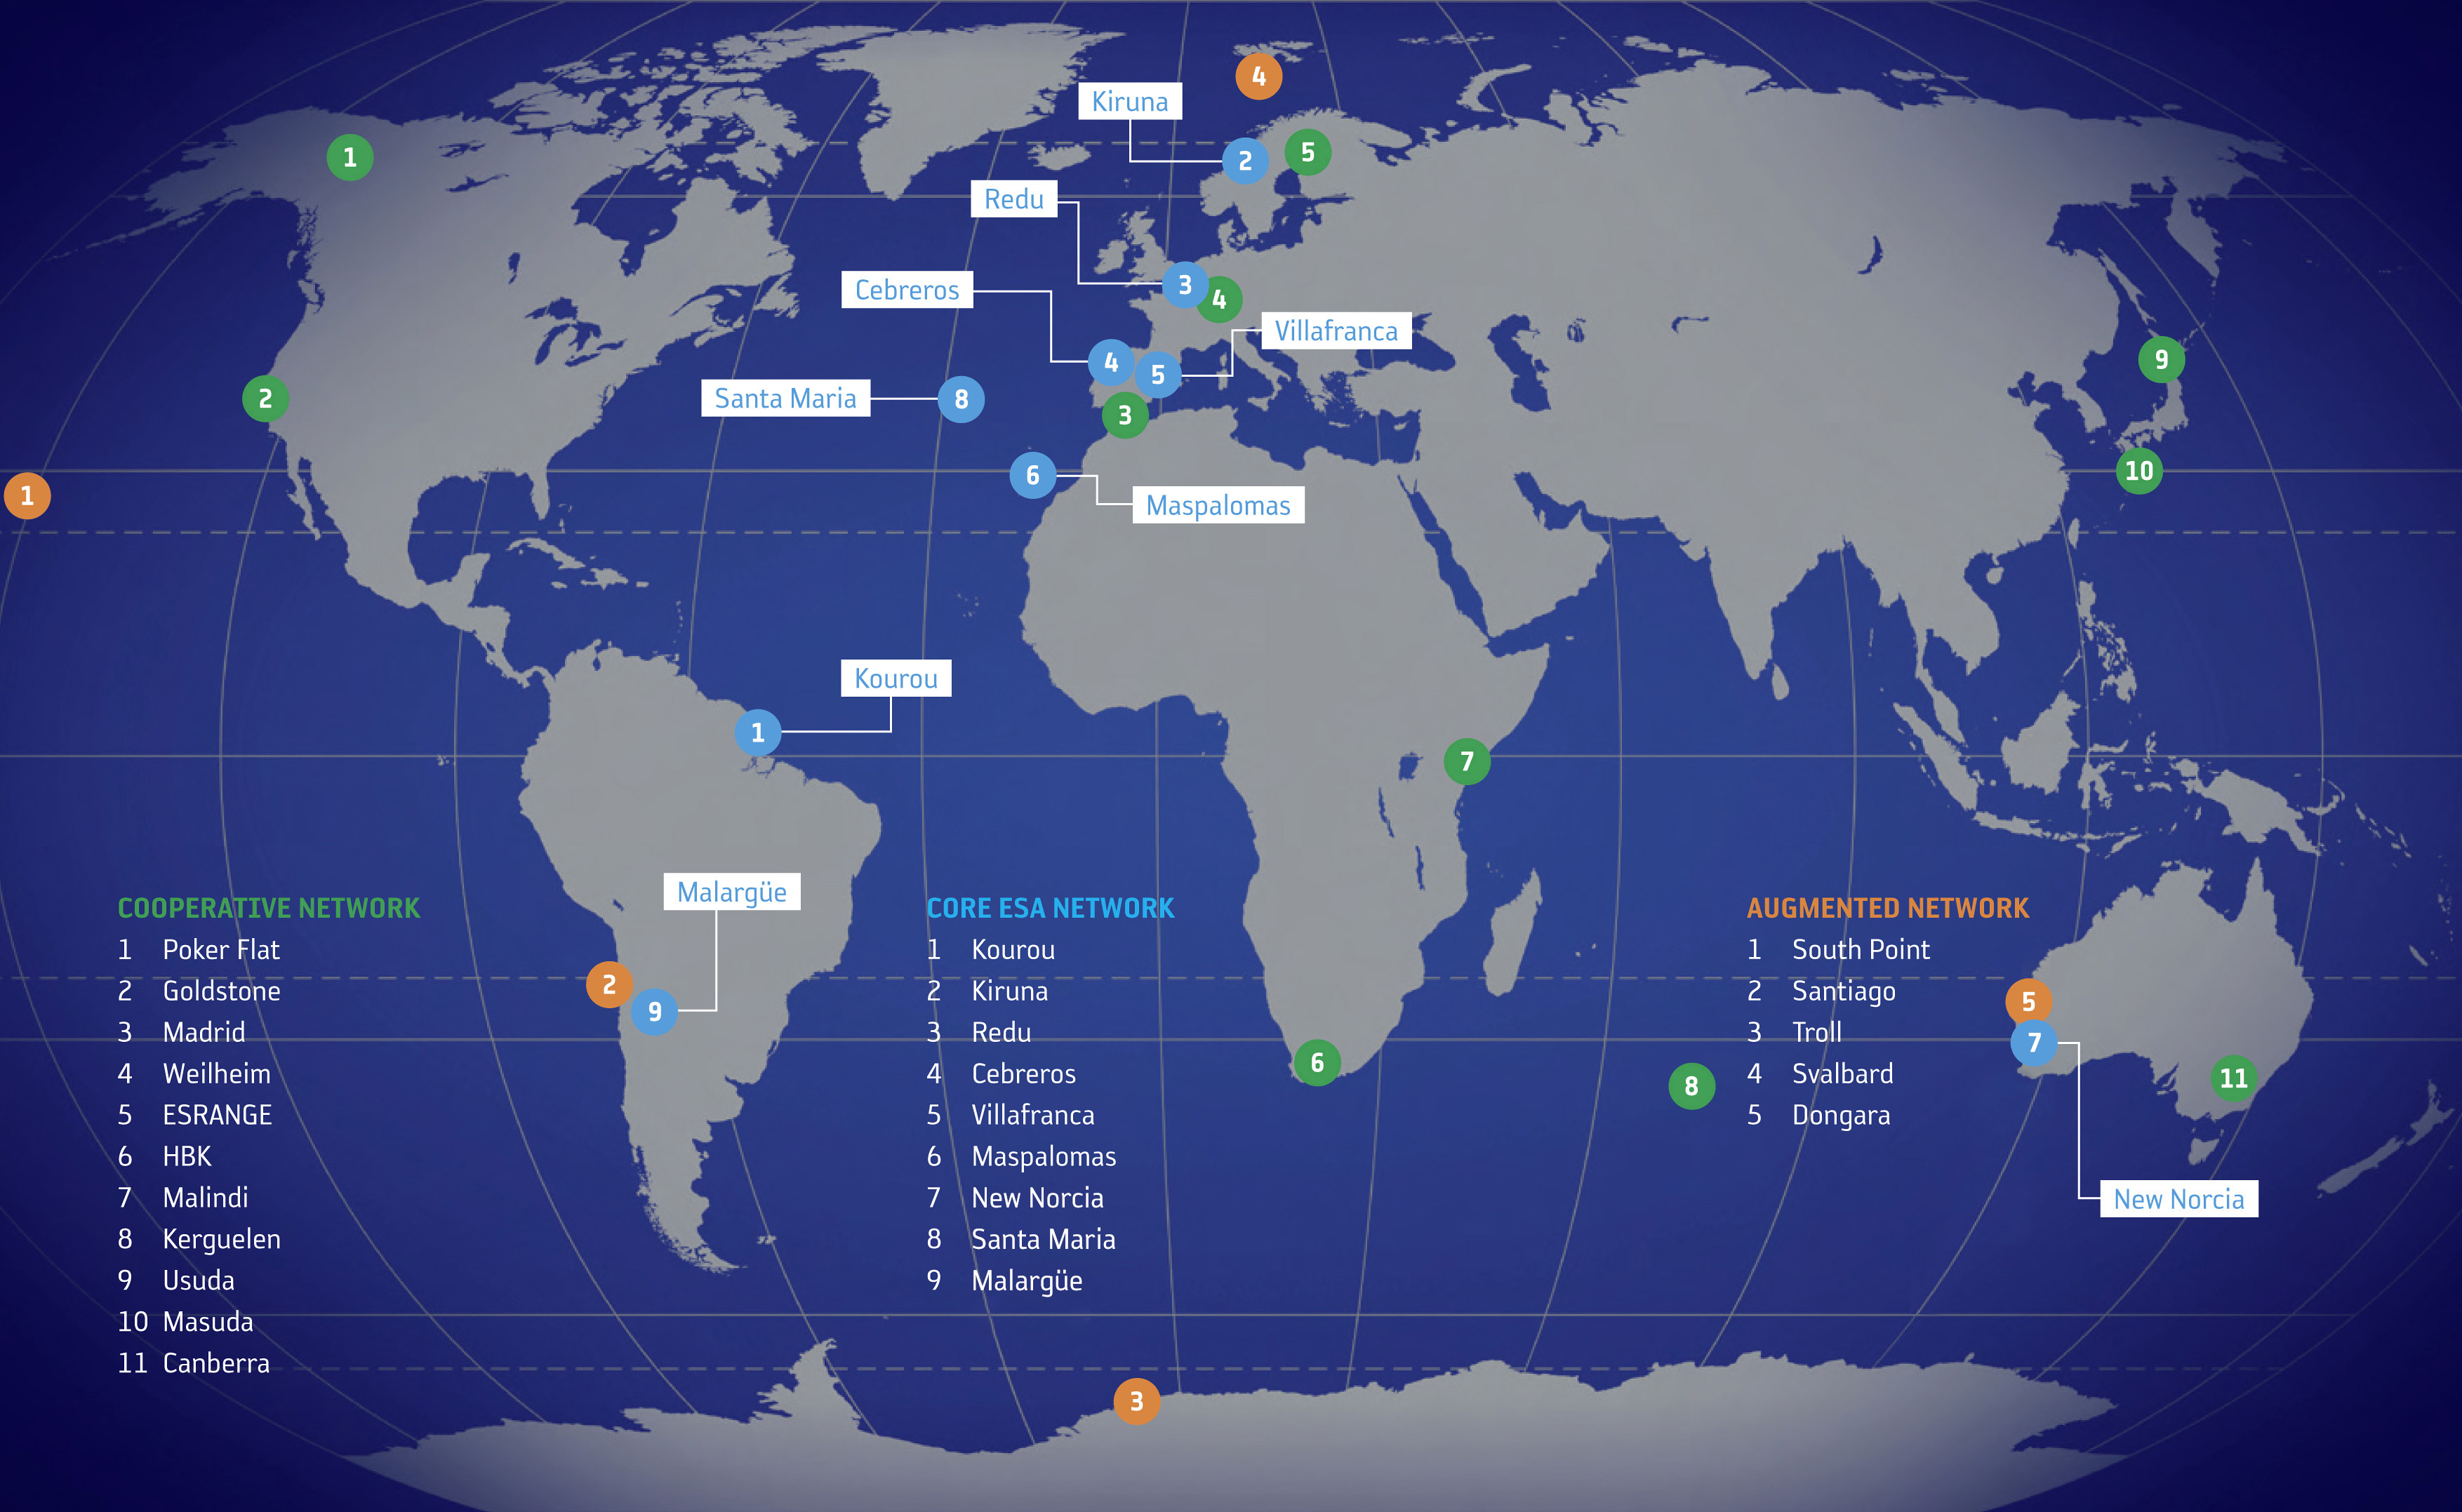
\includegraphics[scale=0.6]{./img/Network_map}
\newline
\newline
Once the latitude is decided, it is also important to have the surroundings clear. High trees can lower the quality of the received/transmitted signal. Also, if the place is very noisy in terms of radio frequencies, it can also cause interferences.
That is why it is good to place the GS in an elevated place, somehow far from big cities.
\section{Parts of a Ground Station}
The GS will be composed of the following parts:
\begin{itemize}
\item \textbf{Antenna:} For \textbf{Astrea} constellation it will be required to use a parabolic antenna as the ground oriented antennas of the satellite nodes operate in \textbf{L band} (1 - 2 GHz). Since these are in the \textbf{microwave} category, the antenna has to be very accurately pointed.
\item \textbf{Transciever:} It is responsible of receiving the signal from the antennas or emitting it to them. Depending on its kind, it can interpret or generate (respectively) that signal, or it can just be seen as an ADC. As far as the last option, the \textbf{Software Defined Radio} should be considered as it provides high versatility with a great bandwidth.
\item \textbf{Rotors system for pointin the antenna:} These should be feeded with the satellite position and they have to point the antenna towards it. Therefore, a link between the received signal going trough to computer and then back to the rotors should be established.
\item \textbf{Computer for signal generating and interpreting}
\end{itemize}

\section{Technical Issues}
The difficulties here are in the reliability requirement. The \textbf{doppler} effect has to be taken into account.

Moreover, since the orbit of the satellites change in time, the GS is usually used for obtaining the new TLE to use later for propagation. This is a bit complex and has to be studied.

\section{Legalities}
There is a license that has to be obtained for the ground station.
Furthemore, the operators of the GS also have to be licensed.
There are limitations in terms of bandwidth and power that have to be respected. \textbf{ITU} is the organism that is also responsible for the frequency allocation.
\end{document}
